% !TeX program = xelatex
% !TeX encoding = UTF-8
\documentclass[UTF8]{standalone}
\usepackage{amsmath,fourier,ctex,tikz,upgreek}
\begin{document}
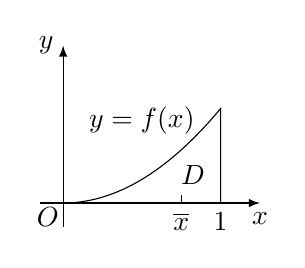
\begin{tikzpicture}
	\draw[-latex] (-0.3,0) node[left=-3pt,below=-2pt] {$O$} -- (2.5,0) node[below] {$x$};
	\draw[-latex] (0,-0.3) -- (0,2) node[left] {$y$};
	\draw[domain=0:2] plot (\x,{0.3*\x^2}) -- (2,0) node[below] {$1$};
	\draw (1.5,0) node[below] {$\overline{x}$} -- ++ (0,0.1);
	\node at (1.65,0.35) {$D$};
	\node[above=2pt] at (1,{0.3*1.5^2}) {$y = f(x)$};
\end{tikzpicture}
\end{document}